\documentclass[a4paper,12pt,floatssmall]{scrartcl}

% Page geometry's formatting
\usepackage[left=2.5cm,right=2.5cm,top=2.5cm,bottom=2.5cm]{geometry}
\usepackage{indentfirst}
\usepackage{placeins}
\usepackage{float}
% Language-specific settings
\usepackage[T1]{fontenc}
\usepackage[utf8]{inputenc}
\usepackage[polish]{babel}
\usepackage{polski}
% Elements' embedding
\usepackage{listings}
\usepackage{graphicx}
\usepackage[bf]{caption}
\usepackage{subcaption}
\usepackage{hyperref}
% Text-formatting
\usepackage[autostyle]{csquotes}
\usepackage{caption}
\usepackage{moresize}
\usepackage{amsmath}
% Miscellaneous
\usepackage[backend=biber,style=ieee]{biblatex}
\usepackage[enable]{easy-todo}
\usepackage{lipsum}
\usepackage{setspace}


% ================================================================================================================================== %
% --------------------------------------------------------- Configuration ---------------------------------------------------------- %
% ================================================================================================================================== %

% Unordered list
\renewcommand{\labelitemi}{\textbullet}

% Bibliography file
\addbibresource{bibliography.bib}

% ================================================================================================================================== %
% ------------------------------------------------------- Macrodefinitions --------------------------------------------------------- %
% ================================================================================================================================== %

% Redefininiton of the title page
\renewcommand{\maketitle}{
\begin{titlepage}
    \vfill
    \begin{center}
        \begin{figure}
            \centering
            
\includegraphics[scale=0.9]{img/header.png}
            \vspace{0.5cm}
        \end{figure}
    \end{center}
    \vspace{2cm}
    \begin{center}
        {\HUGE {\textbf{Programowanie kładów FPGA}}}\\
        \vspace {0.4cm}
        {\Large {(projekt)}}
    \end{center}
    \vspace{4cm}
    \begin{center}
        {\setstretch{1.5}\textbf{\LARGE Implementacja algorytmów cyfrowego przetwarzania sygnałów audio na bazie układu FPGA z interfejsem UART}}
        \vspace{3cm}
    \end{center}
    \vfill
    \begin{center}
        {\textbf{\normalsize Pierczyk Krzysztof}}
    \end{center}
    \vfill
    \begin{center}
        \large{Warszawa, \today \par}
    \end{center}
\end{titlepage}
}

% Definition of `part` module
\renewcommand\partheadstartvskip{\clearpage\null\vfil}
\renewcommand\partheadmidvskip{\par\nobreak\vskip 20pt\thispagestyle{empty}}
\renewcommand\partheadendvskip{\vfil\clearpage\setcounter{section}{0}}
\renewcommand\raggedpart{\centering}

% ================================================================================================================================== %
% ------------------------------------------------------------- Text --------------------------------------------------------------- %
% ================================================================================================================================== %

\begin{document}
    
% Title
\maketitle

% Table of content
\tableofcontents

% Chapter I - Theoretical analysis
\part{Analiza teoretyczna}
\section{Wstęp}

Celem projektu jest opracowanie i~zaimplementowanie zestawu wybranych metod przetwarzania sygnałów audio znanych z~popularnych multiefektów gitarowych. Zadaniem tego typu rozwiązań jest modyfikowanie próbkowanego dźwięku w~czasie rzeczywistym w taki sposób, aby urozmaicić jego brzmienie np. poprzez modulację, przesunięcie fazowe lub wprowadzenie dodatkowych składowych. Przykładami takich efektów są m.in.

\begin{itemize}
    \item \textbf{echo} (opóźnienie, ang. \textit{delay}) - do sygnału dodawana jest jedna lub kilka jego kopii opóźnionych o~określoną liczbę próbek; efekt ma symulować warunki panujące w~halach widowiskowych
    \item \textbf{overdrive} - nazwa ogółu metod prowadzących do znacznego zniekształcenia sygnału bazowego; jednym z~popularnych sposobów jego implementacji jest nałożenie obustronnych ograniczeń na wyjściowe wartości przepuszczanego sygnału
    \item \textbf{flanger} - kolejny efekt wykorzystujący opóźnione próbki sygnału; w~tym przypadku wielkość opóźnienia podlega cyklicznym zmianom, co przekłada się na pulsacyjny charakter wyjściowego dźwięku
    \item \textbf{tremolo} - efekt modulujący amplitudę sygnału zgodnie z~przebiegiem pewnej funkcji okresowej (np. sinus lub fala trójkątna); jego celem jest symulowanie rodzaju artykulacji polegającego na szybkim wydobywaniu dźwięków o~tej samej częstotliwości (np. poprzez szybkie szarpanie pojedynczej struny gitarowej) 
\end{itemize}

Powyższe efekty stanowią jedynie niewielki wycinek stosowanych rozwiązań, wśród których wymienić można także szeroko pojęte metody equalizacji, czy modyfikowania częstotliwości sygnału. Minimalna wersja projektu zakłada implementację scharakteryzowanych metod przetwarzania wraz z~prostymi mechanizmami wprowadzania i~wyprowadzania danych z~urządzenia a~także dostosowywania parametrów filtrów. Jako metodę komunikacji wybrano popularny (choć może w~niec innych zastosowaniach) interfejs UART (ang. \textit{universal asynchronous receiver-transmitter}). Jego prostota umożliwi przyspieszenie procesu implementacji, a~co za tym idzie szybsze przejście do zasadniczej części projektu. Cyfrowy charakter UARTa pozwoli w~przyszłości przejść na popularny interfejs $I^{2}S$, dzięki któremu możliwe będzie proste dołączenie do urządzenia układów przetwornikowych. Testowanie urządzenia obywać się będzie z~pomocą prostej aplikacji w~języku Python, która za pośrednictwem wirtualnego portu szeregowego wysyłać będzie do urządzenia próbki dźwięku. Sygnał wychodzący z~układu FPGA będzie następnie odtwarzany za~pomocą jednej z~wielu dostepnych w~Pythonie bibliotek audio jak np. \verb|pyaudio|.

\section{Analiza interfejsu komunikacyjnego}

Interfejs UART jest dzisiaj dostępny w~niemal wszystkich obecnych na mikrokontrolowerowych oraz w~wielu układach typu SoC. Jego popularność wynika zarówno z~(jak sama nazwa wskazuje) uniwersalnego charakteru jak i~prostoty implementacji. UART to cyfrowe urządzenie peryferyjne umożliwiające szeregową komunikację asynchroniczną. W~większości implementacji parametry komunikacji takie jak szybkość, czy format danych mogą być konfigurowane poprzez zmianę wartości odpowiednich rejestrów sterujących. Nierzadko możliwe jest też ustawienie trybu komunikacji spośród \textit{simplex}, \textit{duples} lub ~\textit{half-duples}. Interfejsy tego typu, szczególnie w~zastosowaniach przemysłowych, są często sprzęgane z~konwerterami poziomów logicznych odpowiednich dla standardów RS-232 lub RS-485.

\begin{figure}
    \centering
    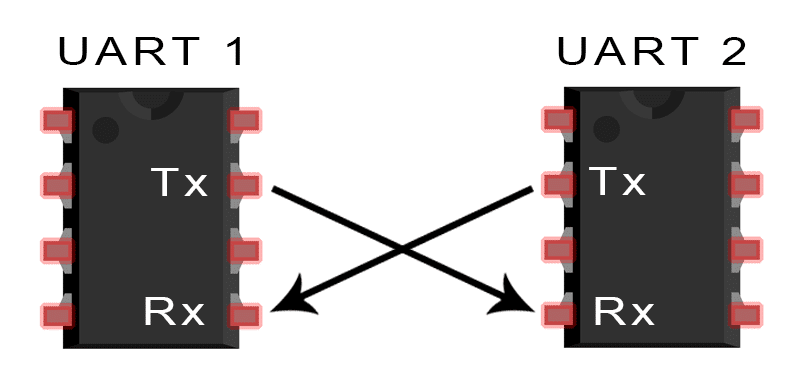
\includegraphics[scale=0.5]{img/uart.png}
    \captionsetup{format=plain,justification=centering}
    \caption{Typowa struktura komunikacji dwóch węzłów z~wykorzystaniem układu UART, źródło: \cite{uart}}
    \label{UART}
\end{figure}

Komunikacja asynchroniczna wymaga aby wszystkie węzły nadawały i~odbierały dane o~z~góry ustalonym formacie i~długości znaku (wynikającym z~szybkości transmisji). Ponadto należy wziąć pod uwagę, że zegary obecne w~poszczególnych urządzeniach mogą się z~czasem rozsynchronizowywać, a~co za tym idzie konieczny jest mechanizm ponownej synchronizacji. W~przypadku komunikacji z~wykorzystaniem modułu UART mechanizm ten wynika z~formatu przesyłanych danych. Typowa ramka składa się z~trzech elementów: \textbf{bitu startu}, \textbf{bitów danyc} oraz \textbf{bitów stopu}. Bit startu oznacza początek nowej ramki i~jest sygnalizowany stanem niskim na linii. Po nim następować może pewna liczba bitów danych - zazwyczaj $7$ lub $8$  - a~na końcu jeden lub dwa bity stopu (sygnalizowane stanem wysokim). Bit startu odpowiada za synchronizację zegarów wykorzystywanych do próbkowania stanu linii, natomiast bity stopu definiują minimalną przerwę między kolejnymi ramkami. Fakt że każdy bit startu to ponowna okazja do zsynchronizowania zegarów sprawia, że nie muszą one pracować z~dokładnie tymi samymi szybkościami. Niewielkie różnice nie powodują błędów w~odbiorze danych.

\begin{figure}
    \centering
    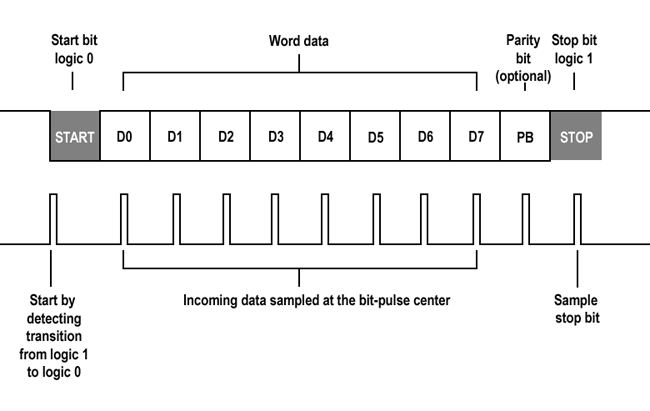
\includegraphics[scale=0.5]{img/uart_frame.png}
    \captionsetup{format=plain,justification=centering}
    \caption{Struktura ramki UART, źródło: \cite{uart_frame}}
    \label{UART}
\end{figure}

Format ramki może zostać rozszerzony o~element kontrolny w~postaci \textbf{bitu parzystości}. Jeśli występuje, przyjmuje on wartość zależną od ilości bitów w~stanie wysokim w~przesyłanych danych i~znajduje się przed bitami stopu. Możliwy jest bit parzystości (ang. \textit{even}) - ustawiony, gdy suma jest parzysta - lub nieparzystości (ang. \textit{odd}) - ustawiany, gdy suma jest nieparzysta. Dodatkowy element pozwala wykrywać ewentualne błędy transmisji. Format ramki często oznacza się w~postaci trzyznakowego identyfikatora postaci $DPS$, gdzie $D$ oznacza ilość bitów danych, $P$ - typ bitu kontrolnego ($E$ - bit parzystości, $O$ - bit nieparzystości, $N$ - brak bitu kontrolnego) a~$S$ ilość bitów stopu. Typowowymi prędkościami transmisji przez UART są:

\begin{itemize}
    \item 9600 bit/s
    \item 19200 bit/s
    \item 38400 bit/s
    \item ...
\end{itemize}

Jest to pewna zaszłość historyczna wynikająca z~częstotliwości standardowych oscylatorów dostępnych na rynku. Moduły współcześnie implementowane w~układach scalonych wzbogacone są często o~dodatkowe wyprowadzenia zegarowe umożliwiające komunikację synchroniczną. Tego typu urządzenia określane są zazwyczaj mianem USART (ang. \textit{universal synchronous asynchronous receiver-transmitter}).

% ================================================================================================================================== %
% ------------------------------------------------------------ Effects ------------------------------------------------------------- %
% ================================================================================================================================== %

\section{Efekty dźwiękowe}

Pierwszą decyzją projektową dotyczącą efektów było stworzenie jednolitego interfejsu implementaowanych bloków przetwarzających. Ma to umożliwić arbitralne połączenie ich w~potok oraz dodanie w~przyszłości nowych efektów bez wprowadzania znacznych zmian w~projekcie. Wykorzystano w~tym celu strukturę zaczerpniętą z~\cite{fpga_pedal}, która została przedstawiona na Rys.\ref{effects-pipe}.

\vspace{0.5cm}
\begin{figure}[ht]
    \centering
    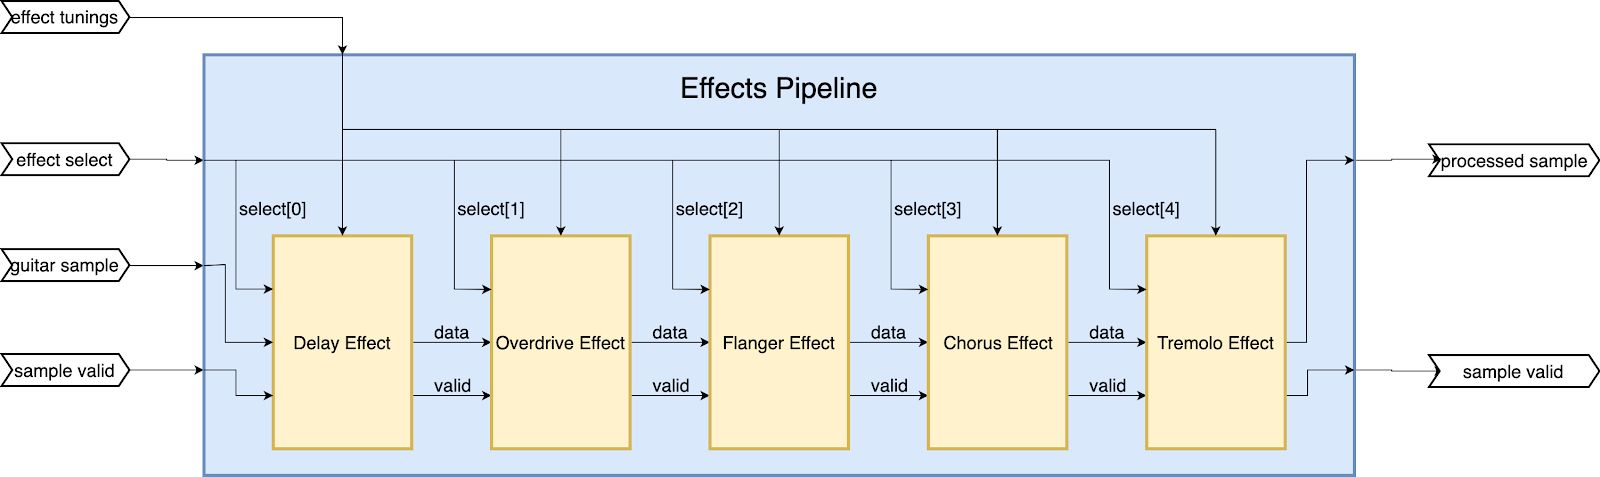
\includegraphics[scale=0.25]{img/pipe.jpg}
    \captionsetup{format=plain,justification=centering}
    \caption{Planowana struktura potoku efektów, źródło: \cite{fpga_pedal}}
    \label{effects-pipe}
\end{figure}
\vspace{0.5cm}

Każdy blok posiada trzy standardowe wejścia oraz dwa standardowe wyjścia. Projekt zakłada wykorzystanie 16-bitowych próbek dźwięku, co determinuje szerokość szyn danych. Wejścia \verb|valid| aktywowane są zboczem narastajacym i~oznaczają pojawienie się nowej próbki na wejściu bloku. Po przetworzeniu próbki moduł ma obowiązek wystawienia danych na linię wyjściową oraz wygenerowanie zbocza narastającego na wyjściu \verb|valid|, które podłączone jest do odpowiadającego wejścia następnego modułu. Każdy z~bloków posiada także jednobitowe wejście \verb|enable|. Stan niski na tej linii oznacza, że blok powinien przekazywać na swoje wyjście próbkę wejściową bez jej modyfikowania. Każdy blok może dodatkowo implementować arbitralne wejścia konfiguracyjne specyficzne dla działania danego algorytmu. W~przypadku blok \textit{overdrive} może być to na przykład 8-bitowa wartość wzmocnienia sygnału i~16-bitowe wartości górnego i~dolnego nasycenia (szczegóły opisano w~dalszej części dokumentu).

Tak zaprojektowana struktura pozwala w~łatwy sposób modyfikować obecne w~systemie efekty oraz nie nakłada ścisłych ograniczeń na interfejs użytkownika wykorzystywany do ich kontrolowania. Również sposób dostarczania i~odbierania danych z~potoku nie jest dzięki temu ograniczony do konkretnego interfejsu komunikacyjnego.

% ----------------------------------------------------------- Overdive ------------------------------------------------------------- %

\subsection{Overdrive}

Jak nakreślono we wstępie efekt przesterowania (ang. \textit{overdive}) określa zespół metod prowadzących do znacznego zniekształcenia sygnału bazowego poprzez dodanie do niego dodatkowych składowych harmonicznych. Częstym sposobem implementacji takiego efektu jest obustronne przycinanie sygnału wejściowego. W~niniejszym projekcie zastosowana zostanie struktura przedstawiona na Rys. {effects-overdrive}.

\vspace{0.5cm}
\begin{figure}[ht]
    \centering
    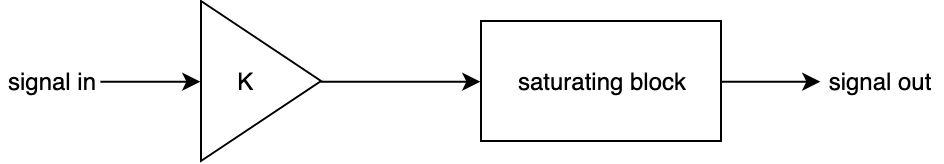
\includegraphics[scale=0.4]{img/overdrive.jpg}
    \captionsetup{format=plain,justification=centering}
    \caption{Schemat bloku \textit{overdrive}, źródło: \cite{fpga_pedal}}
    \label{effects-overdrive}
\end{figure}
\vspace{0.5cm}

Pierwszym etapem przetwarzania jest tutaj wzmocnienie sygnały wejściowego o~wartość kontrolowaną przez rejestr wejsciowy bloku. Zakres potencjalnego wzmocnienia zostanie ustalony na etapie testowania układu. Będzie ono realizowane poprzez 16-bitowe mnożenie z~nasyceniem. Wzmocniony sygnał zostaje następnie przepuszczony przez blok nasycenia. Jeżeli jego wartość mieści się pomiędzy skonfigurowanymi poziomami zostaje on podany na wyjście bez dalszych modyfikacji. W~przeciwnym wypadku na wyjściu pojawia się odpowiednia wartość nasycenia. Funkcjonalność ta może zostać zaimplementowana przy użycia dwóch 16-bitowych komparatorów oraz multipleksera.

% ------------------------------------------------------------ Delay --------------------------------------------------------------- %

\subsection{Delay}

Efekt pogłosu uzyskiwany jest poprzez sumowanie przychodzących próbek z~próbkami opóźnionymi o~określoną liczbę cykli. Realizacja takiego bloku może bazować na filtrze typu FIR (ang. \textit{Finite Impulse Response}) lub IIR (ang. \textit{Infinite Impulse Response}). W~przypadku pierwszego z~nich przeszłe próbki są opóźnionymi wersjami \textbf{sygnału wejściowego}. Liczba próbek sumowanych może być stała lub parametryzowana. Drugi sposób implementacji przewiduje sumowanie pórbki wejściowej jedynie z~jedną wersją opóźnioną sygnału. Wersja ta jest jednak pobierana z~\textbf{wyjścia układu}, co oznacza, że jest ona zależna od wszystkich poprzednich próbek sygnału. Właśnie to rozwiązanie zostanie zastosowane w~niniejszym projekcie. Jego struktura została przedstawiona na Rys.\ref{effects-delay}. W~celu uzyskania stabilnego układu konieczne jest wprowadzenia tłumienia sygnału opóźnionego. Kierując się informacjami zawartymi w~\cite{fpga_pedal} wartości tego tłumienia przyjęto w~zakresie od $0$ do $0.5$. W~celu otrzymania takiego zakresu wyjście z~bloku mnożącego będzie przepusówane o~8~bitów w~prawo (tj. dzielone przez 256).

\vspace{0.5cm}
\begin{figure}[ht]
    \centering
    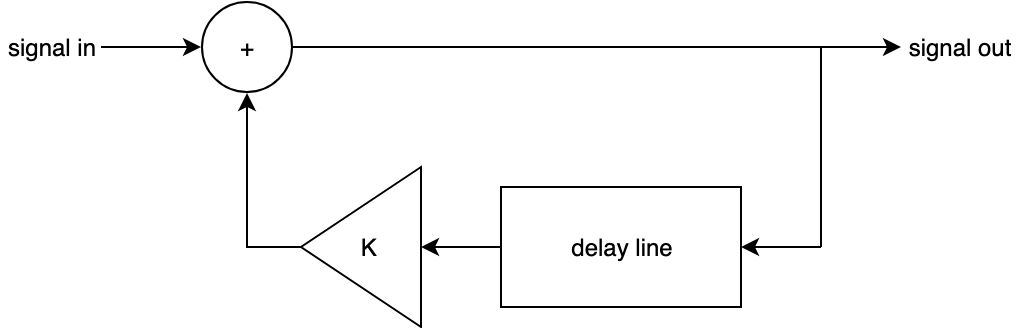
\includegraphics[scale=0.4]{img/delay.jpg}
    \captionsetup{format=plain,justification=centering}
    \caption{Schemat bloku \textit{delay}, źródło: \cite{fpga_pedal}}
    \label{effects-delay}
\end{figure}
\vspace{0.5cm}

Od strony technicznej implementacyja takiego bloku wymaga układu mnożącego, kolejki typu FIFO oraz multipleksera. Siła tłumienia echa ustalana jest poprzez wartość jednego z~wejść do układu mnożącego. Głębokość echa definiuje z~kolei indeks rejestru w~kolejce, którego wartość wystawiana jest na wyjście modułu opóźniającego. Oba parametry efektu regulowane będą przez rejestry wejściowe bloku. Maksymalna głębokość kolejki zostanie ustalona na etapie testowania.

% ----------------------------------------------------------- Flanger -------------------------------------------------------------- %

\subsection{Flanger}

\textit{Flagner} jest efektem, którego brzmienie trudno opisać, jednak zasada jego działania jest stosunkowo prosta. Efekt ten powstaje poprzez nałożenie na sygnał filtru grzebieniowego, którego charakterystyka amplitudowa wykonuje sinusoidalne oscylacje w~okół ustalonego punktu. W~prakyce układ taki realizuje się poprzez sumowanie sygnału z~jego opóźnionymi (nieprzetworzonymi) wersjami. Wartość tego opóźnienia jest jednak okresowo zmienna. Struktura takiego rozwiązania przedstawiona została na Rys.\ref{effects-flanger}. Aby kontrolować siłę efektu do ukłądu wprowadzone zostaną dodatkowe bloki tłumienia. Ich wartość zawierać się będzie w~przedziale od $0$~do $1$, natomiast ich suma będzie stale równa $1$. Podobnie jak w~przypadku pogłosu wykorzystywana głębokość kolejki FIFO (a~tym samym efektywna amplituda oscylacji wartości opóźnienia) będzie ustalana porpzez zewnętrzny parametr.

\vspace{0.5cm}
\begin{figure}[ht]
    \centering
    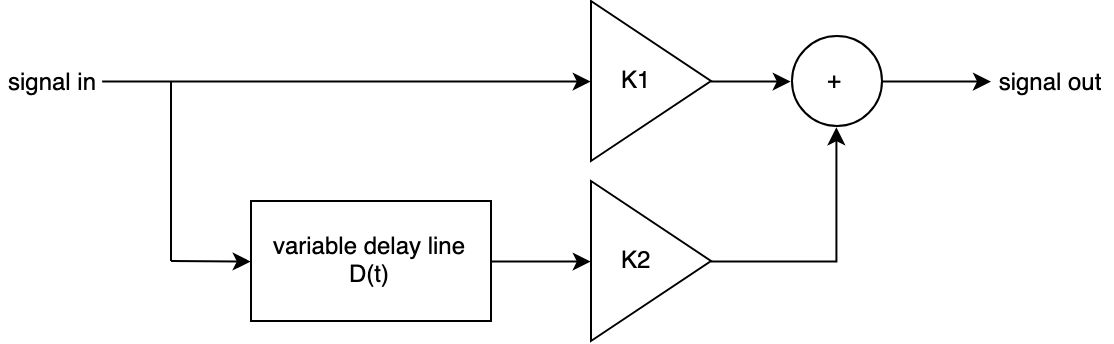
\includegraphics[scale=0.4]{img/flanger.jpg}
    \captionsetup{format=plain,justification=centering}
    \caption{Schemat bloku \textit{flanger}, źródło: \cite{fpga_pedal}}
    \label{effects-flanger}
\end{figure}
\vspace{0.5cm}

Implementacja efektu będzie wykorzystywac bloki stworzone podczas realizacji poprzedniego efektu takie jak układy mnożące oraz kolejka FIFO. Dodatkowym elementem będzie tutaj generator funkcji sinus o~zmiennej częstotliwości. Czestotliwość ta będzie również ustalana poprzez zewnętrzny parametr.

% ----------------------------------------------------------- Tremolo -------------------------------------------------------------- %

\subsection{Tremolo}

Efekt tremolo uzyskuje się poprez modulację amplitudy sygnału wejściowego. Jest to realizowane poprzez mnożenie sygnału z~pewną funkcją okresową jak np. sinus lub fala trójkątna. W~projekcie zaimplementowane zostaną oba rodzaje modulacji. Po wykonaniu testów wybrany zostanie ten, który będzie pozwalał uzyskać ciekawsze brzmienie. Schemat blokowy rozwiązania został przedstawiony na Rys.\ref{effects-tremolo}. Podobnie jak w~przypadku pogłosu wykorzystane zostanie tu 8-bitowe przesówanie wyniku mnożenia celem uzyskania efektywnej amplitudy fali modulującej w~zakresie od $0$ do $1$ (przy załżeniu, że wyjście z~generatora fali ma wartość 8-bitową).

\vspace{0.5cm}
\begin{figure}[ht]
    \centering
    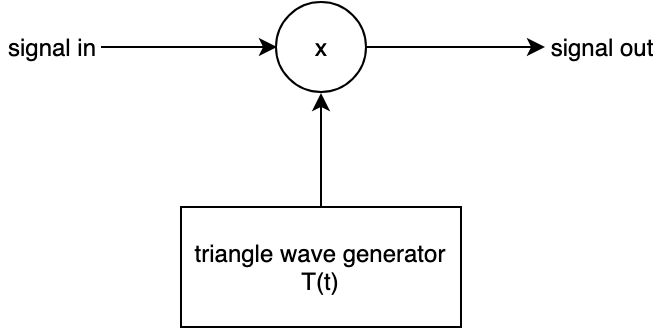
\includegraphics[scale=0.4]{img/tremolo.jpg}
    \captionsetup{format=plain,justification=centering}
    \caption{Schemat bloku \textit{tremolo}, źródło: \cite{fpga_pedal}}
    \label{effects-tremolo}
\end{figure}
\vspace{0.5cm}
% ================================================================================================================================== %
% ---------------------------------------------------------- Interface ------------------------------------------------------------- %
% ================================================================================================================================== %

\section{Interfejs użytkownika}

Ostatnim elementem projektu jest zaimplementowanie wygodnego interfejsu użytkownika. Powinien on umożliwiać niezależną aktywację każdego z~efektów oraz pozwalać na regulowanie ich parametrów. Układ FPGA udostępniać będzie cztery wejścia cyfrowe (przyciski). Zostaną one podłączone (za pośrednictwem przerzutników) do wejść \verb|enable| poszczególnych bloków przetwarzających. Aktywacja efektu możliwa będzie dzięki zmianie stanu przełącznika. Kontrola parametrów bloków przetwarzana zostanie zrealizowana za pomocą potencjometrów. Ich interfejs może zostać stworzony na dwa sposoby. Ostateczny wybór zostanie podjęty po głęszbym przeanalizowaniu zagadnienia. 

Pierwszym pomysłem jest wykorzystanie modułu XADC od Xilinx. Pozwoliłoby to na podłączenie wszystkich potencjometrów do układu FPGA z~wykorzystaniem multipleksera analogowego (np. CD74HC4067), którego wejście przełączane byłoby z~pewną częstotliwością przez układ sterujący. Wymagałoby to jednak wykorzystanie gotowego bloku IP oraz stworzenia odpowiedniego interfejsu od strony aplikacji.

Drugim pomysłem jest wdrożenie dodatkowego modułu UART, który komunikowałby się z~zewnętrznym mikrokontrolerem realizującym pomiar napięć na potencjometrach poprzez wbudowane kanały przetwornika A/C. W~takim przypadku układ FPGA odpytywałby podrzędny względem niego mikrokontroler w~sposób cykliczny, pozyskując cyfrowe wartości orientacji potencjometrów. Niezależnie od wyboru metody cyfrowe wartości pomiarów zostaną podłączone poprzez przerzutniki do wejśc konfiguracyjnych odpowiendich bloków przetwarzających sygnały.

% ================================================================================================================================== %
% --------------------------------------------------------- Simulations ------------------------------------------------------------ %
% ================================================================================================================================== %

\section{Planowane symulacje}

Planowane symulacje można podzielić na dwie zasadnicze kategorie. Pierwsza z~nich obejmuje proste testy jednostkowe \textbf{w~skali mikro}. Mowa tu o~modułach takich jak generator taktowania dla UARTa, układ mnożący, czy generator fali trójkątnej wykorzystywany w~algorytmach przetwarzania sygnału. Każdemu z~tych elementów powinien odpowiadać prosty podprojekt typu \textit{testbench}, który weryfikuje poprawność jego działania. Chociaż tworzenie tak drobnych elementów symulacyjnych może być do pewnego stopnia uciążliwe przy większej ilości testowanych elementów, to jednak doświadczenie pochodzące z~programowania pokazuje, że pozwala to zapobiec eskalacji wpływu drobnych błędów na działanie systemu jako całości.

Drugą kategorią symulacji będą testy systemowe sprawdzające \textbf{makroskopowe} działanie poszczególnych bloków funkcjonalnych. Tutaj również każdy z~modułów powinien otrzymać dedykowany projekt testowy. W~tym przypadku poza poprawnością działania podsystemów zostanie również zweryfikowana ich wydajność. Oszacowanie czasów przetwarzania danych przez dany blok funkcjonalny oraz jego złożoność przestrzenna (wymagana liczba zasobów układu FPGA) pozwolą z~jednej strony określić warunki krańcowe ich funkcjonowania, a~z~drugiej oszczować potencjalne możliwości rozwoju systemu np. o~dodatkowe efekty.

% ================================================================================================================================== %
% ------------------------------------------------------------ Tests --------------------------------------------------------------- %
% ================================================================================================================================== %

\section{Planowane testy}

Pierwszym testem poprawności działaniu układu będzie oczywiście empiryczna ocena dźwięku uzyskanego za pomocą poszczególnych efektów. Pozwoli ona nie tylko wykryć potencjalne błędy w~algorytmach przetwarzania (objawiające się np. wprowadzaniem nadmiernego szumu), ale także dostosować stałe parametry układu takie jak długości zastosowanych kolejek FIFO. 

Drugi krok weryfikacji rozwiązania zostanie zrealizowany dzięki zastosowanemu interfejsowi danych w~postaci aplikacji języka Python. Fakt, że posiadać będzie ona dostęp zarówno do surowych jak~i przetworzonych danych pozwoli w~łatwy sposób wyrysować wykresy przedstawiające przebiegi sygnałów i~np. ich transformaty. Możliwe będzie dzięki temu dokładne przyjrzenie się efektom działania poszczególnych filtrów celem wykrycia źródeł potencjalnych problemów. 

% ================================================================================================================================== %
% ----------------------------------------------------------- Platform ------------------------------------------------------------- %
% ================================================================================================================================== %

\section{Wybór platformy}

Ostateczny wybór platformy zostanie dokonany po stworzeniu fundamentów projektu pozwalających oszacować wymagania urządzenia dotyczące zasobów układu FPGA. Na ten moment potencjalny wybór został zawężony do trzech zestawów ewaluacyjnych. Pierwszy z~nich to \textbf{Digilent Cmod A7} wyposażony w~moduł XC7A35T-1CPG236C z~rodziny Artix-7. Niewielkie rozmiary oraz cena nieprzekraczająca 400zł są największymi zaletami tego wariantu. Został on wyposażony w~8-bitową pamięć SRAM o pojemności 512KB oraz pamięć szeregową Quad-SPI wielkości 4MB. Druga z~rozważanych platform to \textbf{Digilent Arty S7}. Jest to układ bardziej rozbudowany od poprzedniego. Posiada on na pokładzie moduł XC7S50-1CSGA324C (Spartan-7) zawierający ponad $50\%$ więcej bloków logicznych. Sama płytka oferuje ponadto kilka diod LED, przełączników mono- i~bistabilnych oraz cztery złącza Pmod. Cena tej platformy jest o~około $18\%$ wyższa, co oznacza wysoki stosunek zasobów do ceny, jednak liczyć się trzeba ze znacznie większymi wymiarami płytki.

Trzecim wariantem jest z~kolei zestaw \textbf{Digilent Cora Z7}. Jest to układ najuboższy w~bloki logiczne a~przy tym wyceniany na podobnym poziomie co Arty S7. Posiada on jednak układ XC7Z007S-1CLG400C z~rodziny Zynq co oznacza, że poza modułem FPGA zawiera on również jednordzeniowy procesor w~architekturze ARM Cortex-A9. Zestaw ten brany jest pod uwagę jedynie ze względu na prywatną sympatię autora do mikrokontrolerów bazujących na architekturze Cortex-M i~wynikającej z~niej chęci zapoznania się z~architekturą aplikacyjną rodziny ARM. Wariant ten zostanie wybrany wówacz, jeżeli zasoby zawartego w~nim modułu FPGA okażą się wystarczające do zaimplementowania tworzonego rozwiązania.


% Chapter II - Implementation
\part{Implementacja}
% 4. Bloki DSP
%     - symulacje
% 5. Generatory
%     - trójkątny
%        - schemat blokowy z opisem parameterów
%     - symetryczny
%        - schemat blokowy z opisem parameterów
%     - symulacje
% 6. Efekt `overdrive'
%     - schemat blokowy z opisem parameterów
%     - automat skończony
%     - symulacje
% 7. Efekt `tremolo'
%     - schemat blokowy z opisem parameterów
%     - automat skończony
%     - konfigruacja bloku BRAM
%     - symulacje
% 8. Efekt `delay'
%     - schemat blokowy z opisem parameterów
%     - automat skończony
%     - konfigruacja bloku BRAM
%     - symulacje
% 9. Efekt `flanger'
%     - schemat blokowy z opisem parameterów
%     - automat skończony
%     - konfigruacja bloków BRAM
%     - symulacje
% 10. Potok
%     - konfiguracja
%     - symulacje
% 11. Integracja
%     - symulacje
% 12. Podsumowanie
\section{Struktura projektu}

\vspace{0.5cm}
\begin{figure}[ht]
    \centering
    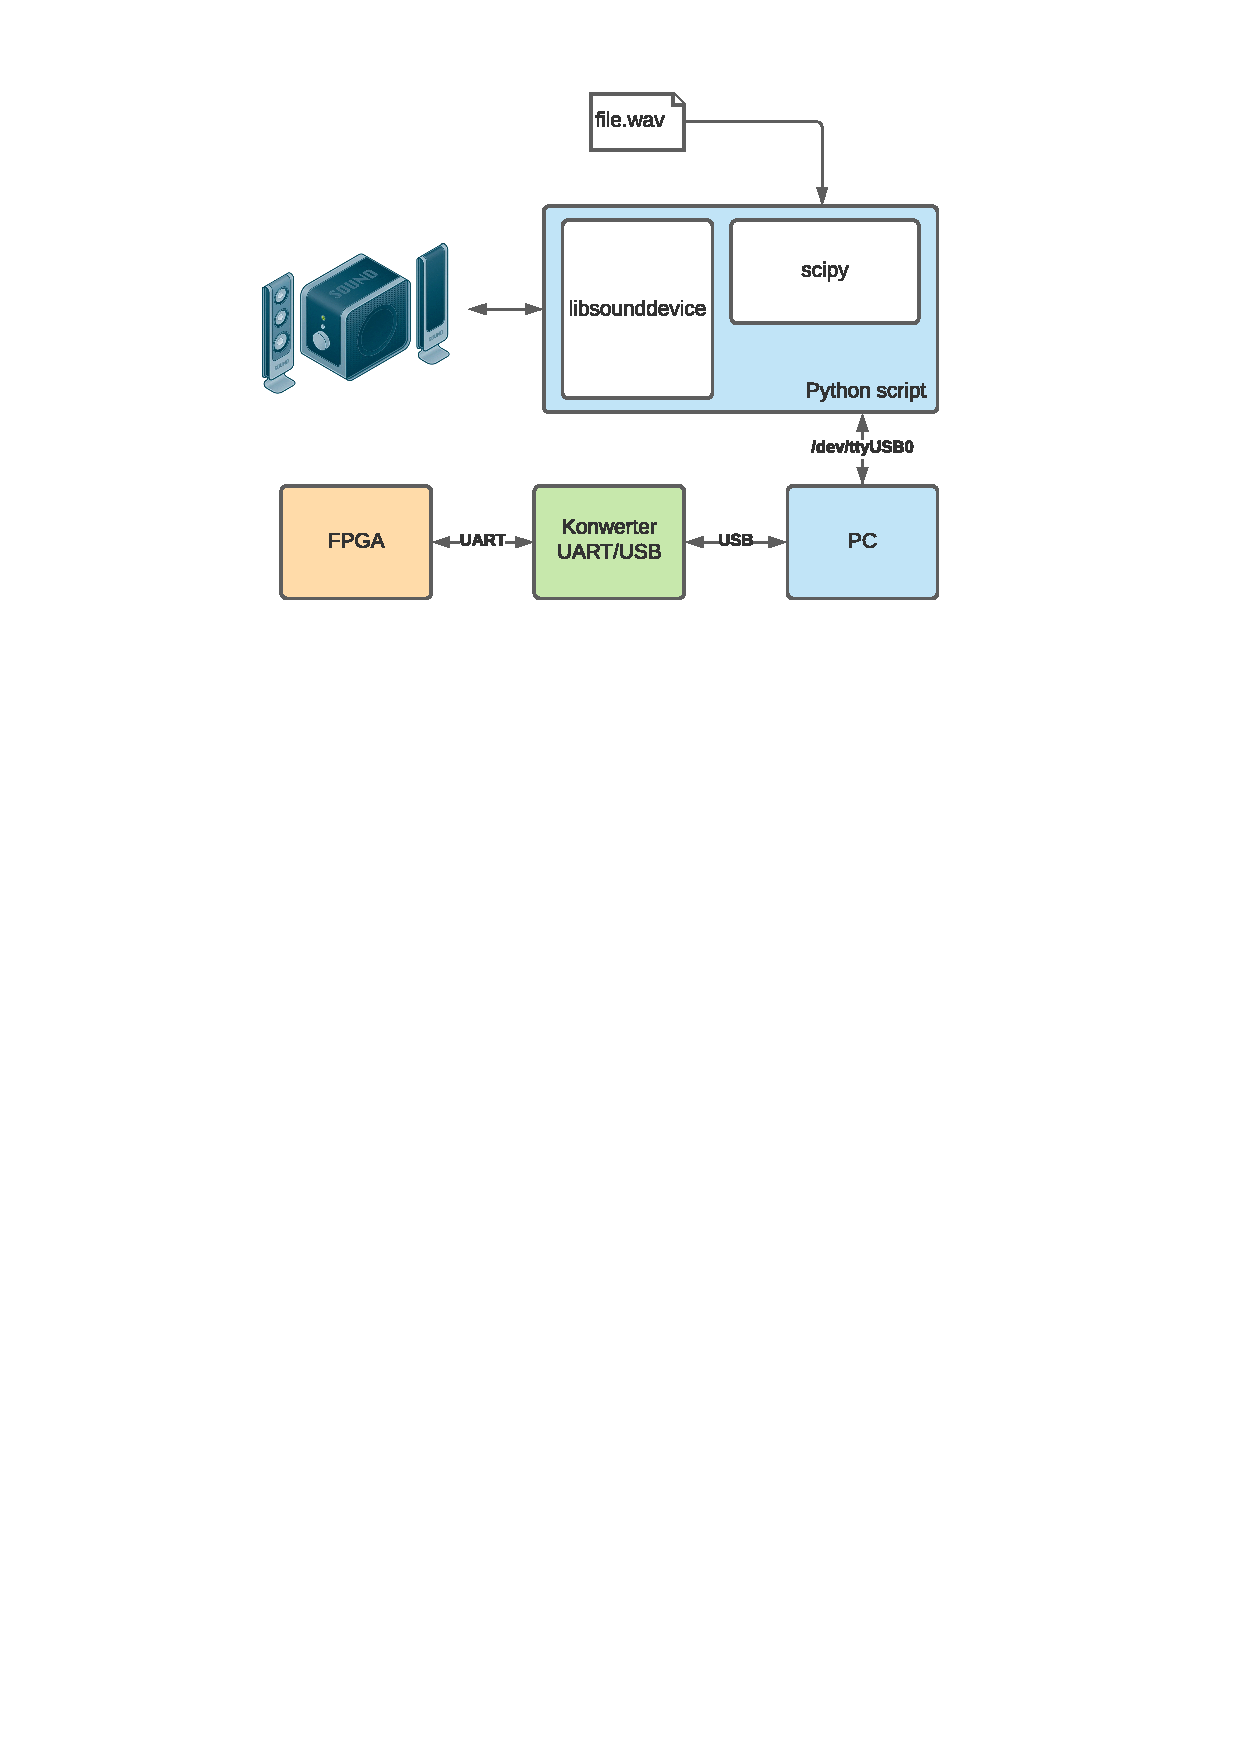
\includegraphics[scale=0.75]{img/diagrams/system.pdf}
    \captionsetup{format=plain,justification=centering}
    \caption{Struktura systemowa projektu}
    \label{system-structure}
\end{figure}
\vspace{0.5cm}

Realizację przedstawionej w~części pierwszej koncepcji rozpoczęto od nakreślenia struktury projektu na trzech płaszczyznach: \textbf{systemowej}, \textbf{implementacyjnej} i~\textbf{projektowej}. Pierwsza z~nich obejmowała zdefiniowanie węzłów, które będą brały udział w~procesie przetwarzania dźwięku od otwarcia zawierajacego go pliku do chwili wyemitowania przetworzonej wersji przez urządzenie audio. Jak przedstawiono na Rys. \ref{system-structure}, wyróżniono cztery zasadnicze jednostki. \textit{Skrypt języka Python} odpowiedzialny jest za załadowanie pliku dźwiękowego do pamięci RAM, przekazanie i~odebranie go z~układu przetwarzającego, a~także wysterowanie domyślnego urządzeni audio w~oparciu o~zmodyfikowane próbki. Urządzeniem przetwarzającym jest oczywiście układ \textit{FPGA}, który implementuje wymienione wyżej filtry. Pośrednikami w~komunikacji pomiędzy układem scalonym a~aplikacją są oparty o~układ FT232R \textit{mostek USB/UART} oraz \textit{komputer klasy PC}. Taka konfiguracja pozwala na dwukierunkową transmisję danych z~prędkością do 375KB na sekundę, co przy założeniu 16-bitowych próbek oraz częstotliwości próbkowania na poziomie 44100Hz powinno wystarczyć do strumieniowania dźwięku zarówno w~trybie mono jak i~stereo. W~projekcie wykorzystano biblioteki \verb|sounddevice| oraz \verb|scipy| języka Python. Pierwsza z~nich udostępnia interfejs dla szerokiej gamy urządzeń audio, natomiast druga pozwala przetwarzać pliki w~formacie WAV do postaci tablic danych biblioteki \verb|numpy|. Aby zredukować czas wykonywania operacji na wirtualnym porcie szeregowym, zdecydowano się podzielić strumieniowane dane na bloki o~wielkości 5000B, które wysyłane są do układu FPGA pojedynczo.

Określenie struktury implementacyjnej obejmowało doprecyzowanie zaproponowanych w~części pierwszej koncepcji konfiguracji urządzenia. Ostatecznie zdecydowano się na model przedstawiony na Rys. \ref{fpga-structure}. Wyróżnić w~nim można cztery zasadnicze części. Odbiornik oraz nadajnik UART zostały wcielone w~ramy dwóch szerszych struktur, które umożliwiają wymianę N-bajtowych próbek danych w~ramach pojedynczej transakcji. W~ramach interfejsu użytkownika wykorzystano moduł XADC (ang. \textit{Xilinx Analog/Digital Converter}), który w~ramach jednostki \verb|AnalogScanner| pozwala konwertować sekwencję do 16 sygnałów analogowych podłączonych do układu poprzez zewnętrzny multiplekser. Umożliwi to dołączenie szeregu potencjometrów odpowiedzialnych za określanie parametrów filtrów przedstawionych w~centralnej części rysunku. Aby zmaksymalizować elastyczność konfiguracji postanowiono pozostać przy pierwotnej koncepcji jednolitego interfejsu efektów, którego szczegóły zostaną omówione w~dalszej części dokumentu. Dodatkowym elementem projektu jest także zestaw rejestrów konfiguracyjnych, które określają porametry interfejsów komunikacyjnych oraz sposób mapowania mierzonych wartości analogowych na parametry filtrów. Na ten moment zostały one zaimplementowane w~sposób niejawny, jednak w~przyszłości planowane jest zmiana tego podejścia na rzecz ułatwienia rekonfiguracji urządzenia.

\vspace{0.5cm}
\begin{figure}[ht]
    \centering
    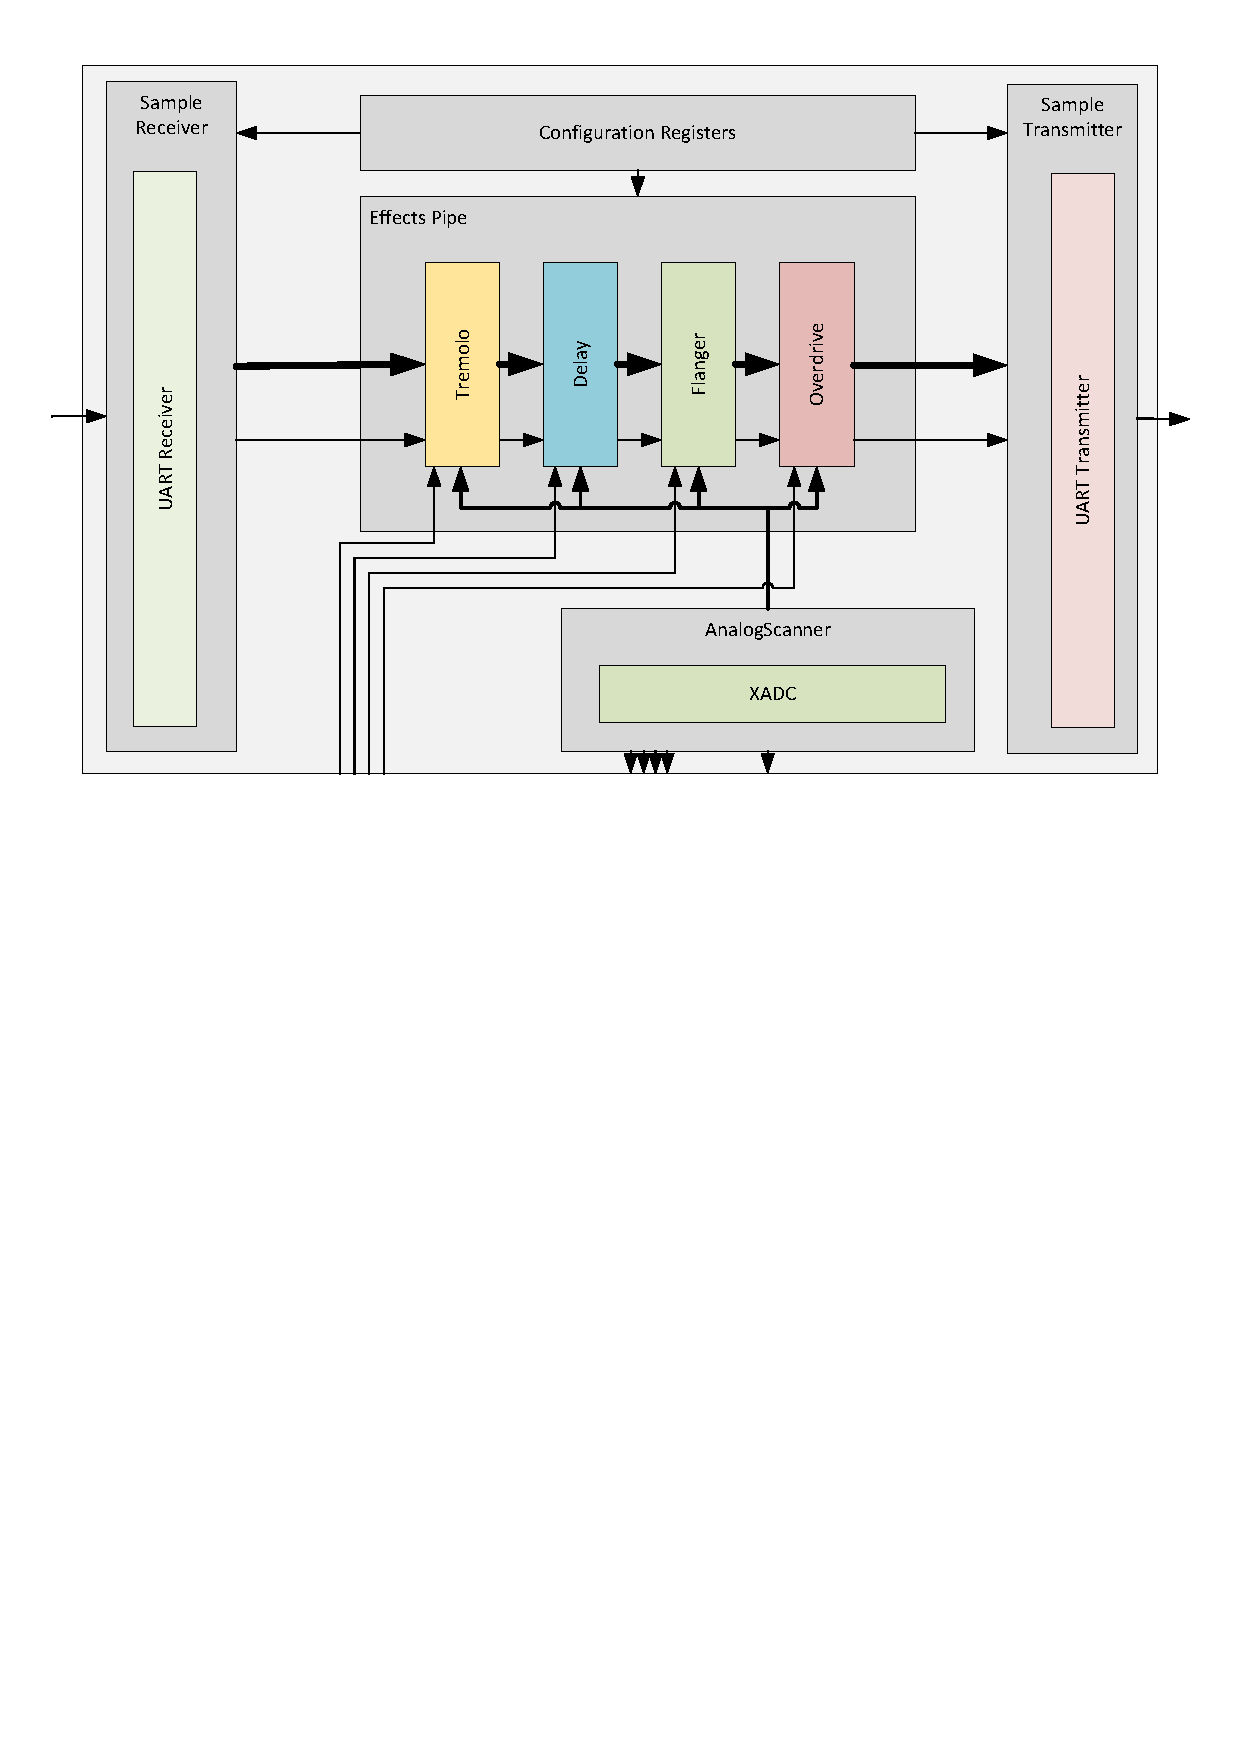
\includegraphics[scale=0.75]{img/diagrams/project_diagram.pdf}
    \captionsetup{format=plain,justification=centering}
    \caption{Struktura implementacyjna projektu}
    \label{fpga-structure}
\end{figure}
\vspace{0.5cm}

Ostatnią - choć nie mniej ważną z~perspektywy projektanta - kwestią wymagającą określenia była struktura samego projektu rozumiana jako podział drzewa plików i~katalogów. Oprogramowanie \textit{Vivado} wykorzystywane na etapie symulacji oraz syntezy nie jest w~opinii autora optymalnym środowiskiem programistycznym\footnote{Vivado jest oczywiście środowiskiem służącym do \textbf{konfiguracji} a~nie programowania układów FPGA. Z~uwagi na brak lepszego terminu postanowiono jednak pozostać przy określeniu \textit{środowisko programistyczne}}. Elementami, które składają się na taki stan rzeczy są m.in. męczący oczy interfejs graficzny oraz brak integracji z~systemami kontroli wersji. Z~tego względu zdecydowano się na wykorzystanie oprogramowania \textit{Visual Studio Code} jako domyślnego narzędzia tworzenia kodu oraz zarządzania projektem. Aby było to możliwe koniecznym stało się zapoznanie się z~odpowiednimi dokumentami (\cite{vivado_design_flow}, \cite{vivado_design_methodology}) udostępnianymi przez firmę Xilinx. Pozwoliło to określić te z~plików generowanych przez \textit{Vivado}, które są konieczne do odtworzenia struktury projektu. Na tej podstawie zdecydowano się na podział przedstawiony na Rys. \ref{project-structure}. Elementami wartymi wyróżnienia są katalogi \textit{src/ip} oraz \textit{workdir}. Pierwszy z~nich przechowuje pliki w~formacie XML opisujące konfigurację wykorzystywanych w~projekcie bloków XADC oraz BRAM (ang. \textit{Block Random Access Memory}), które zostały wyekstrahowane ze struktury projektowej \textit{Vivado}. Drugi stanowi z~kolei miejsce docelowe dla hierarchii plików generowenj przez samo oprogramowanie. Jedynym jej elementem, który włączony został do systemu kontroli wersji jest plik \verb|GuitarMultieffect.xpr| zawierający pełny opis struktury projetktu. Warto zauważyć, że przyjęte podejście do kontroli wersji pozwoli na uruchomienie projektu jedynie przy użyciu aktualnie wykorzystywanej wersji \textit{Vivado} (2020.2).

\vspace{0.5cm}
\begin{figure}[ht]
    \centering
    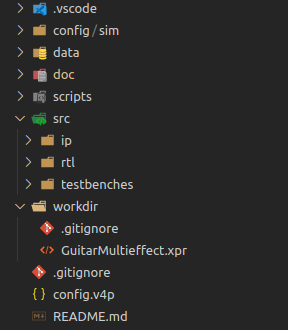
\includegraphics[scale=0.7]{img/source_structure.png}
    \captionsetup{format=plain,justification=centering}
    \caption{Struktura projektowa}
    \label{project-structure}
\end{figure}
\vspace{0.5cm}

\section{Interfejs komunikacyjny}

Budowę interfejsu komunikacyjnego rozpoczęto od zaimplementowania modułów UART. Układ ich wyprowadzeń przedstawiono na Rys. \ref{uart-structure}. Wąskie strzałki symbolizują linie jednobitowe. Strzałki czerwone oraz żółte to linie wielobitowe. Pierwsze z~nich oznaczają, że są port połączony został z~potokiem przetwarzania danych. Z~kolei w~przypadku drugich porty wystawione są poza potok. Konwencja ta została zachowana w~przypadku kolejnych rysunków.

Wejście \verb|clk| to podłączenie do głównego zegara systemowego, natomiast \verb|reset| to asynchroniczny reset układu (aktywny stanem niskim). Wejścia te są uniwersalne dla wszystkich implementowanych modułów. Porty \verb|rate| pozwalają określić szybkość transmisji. Wyrażana jest ona jako ilość cykli zegara systemowego przypadających na jeden znak wysyłany/transmitowany (minus 1). W~przypadku interfejsu odbierającego ustawienie wartości 0~na tym porcie zablokuje odbiór danych\footnote{Stan linii RX testowany jest w~połowie trwania znaku, co wymusza maksymalny stosunek prędkości transmisji do prędkości zegara systemowego na poziomie 1:2}. Oba moduły implementują także linię wyjściową \verb|busy|, która, gdy ustawiona w~stanie wysokim, oznacza, że układ zajęty jest odbiorem/transmisją danych. 

Podsystem odbiorczy udostępnia wyjście odebranych danych \verb|data| oraz oczywiście linię szeregową \verb|rx|. Port \verb|error| reprezentowany jest jako trzybitowa linia typu \verb|record|. Ustawiana jest w~momencie zmiany stanu linii \verb|busy| ze stanu wysokiego na niski i~zawiera flagi błędu odbioru bitu startu, bitów stopu oraz parzystości. Wystąpienie błędu sygnalizowane jest stanem wysokim. Równolegle z~flagami błędów ustawiany jest również port \verb|data|\footnote{W~przypadku wystąpienia błędu odbioru port \textit{data} jest zerowany}. Podsystem nadawczy posiada porty \verb|data| i~\verb|tx| o~znaczeniu analogicznym do przypadku odbiorczego. Udostępnia on także linię \verb|transfer|. Ustawienie jej w~stan wysoki\footnote{Linia aktywna jest \underline{poziomem} wysokim} w~czasie, gdy linia \verb|busy| znajduje się w~stanie niskim, rozpoczyna transmisję danych znajdujących się na wejściu \verb|data|.

\vspace{0.5cm}
\begin{figure}[ht]
    \centering
    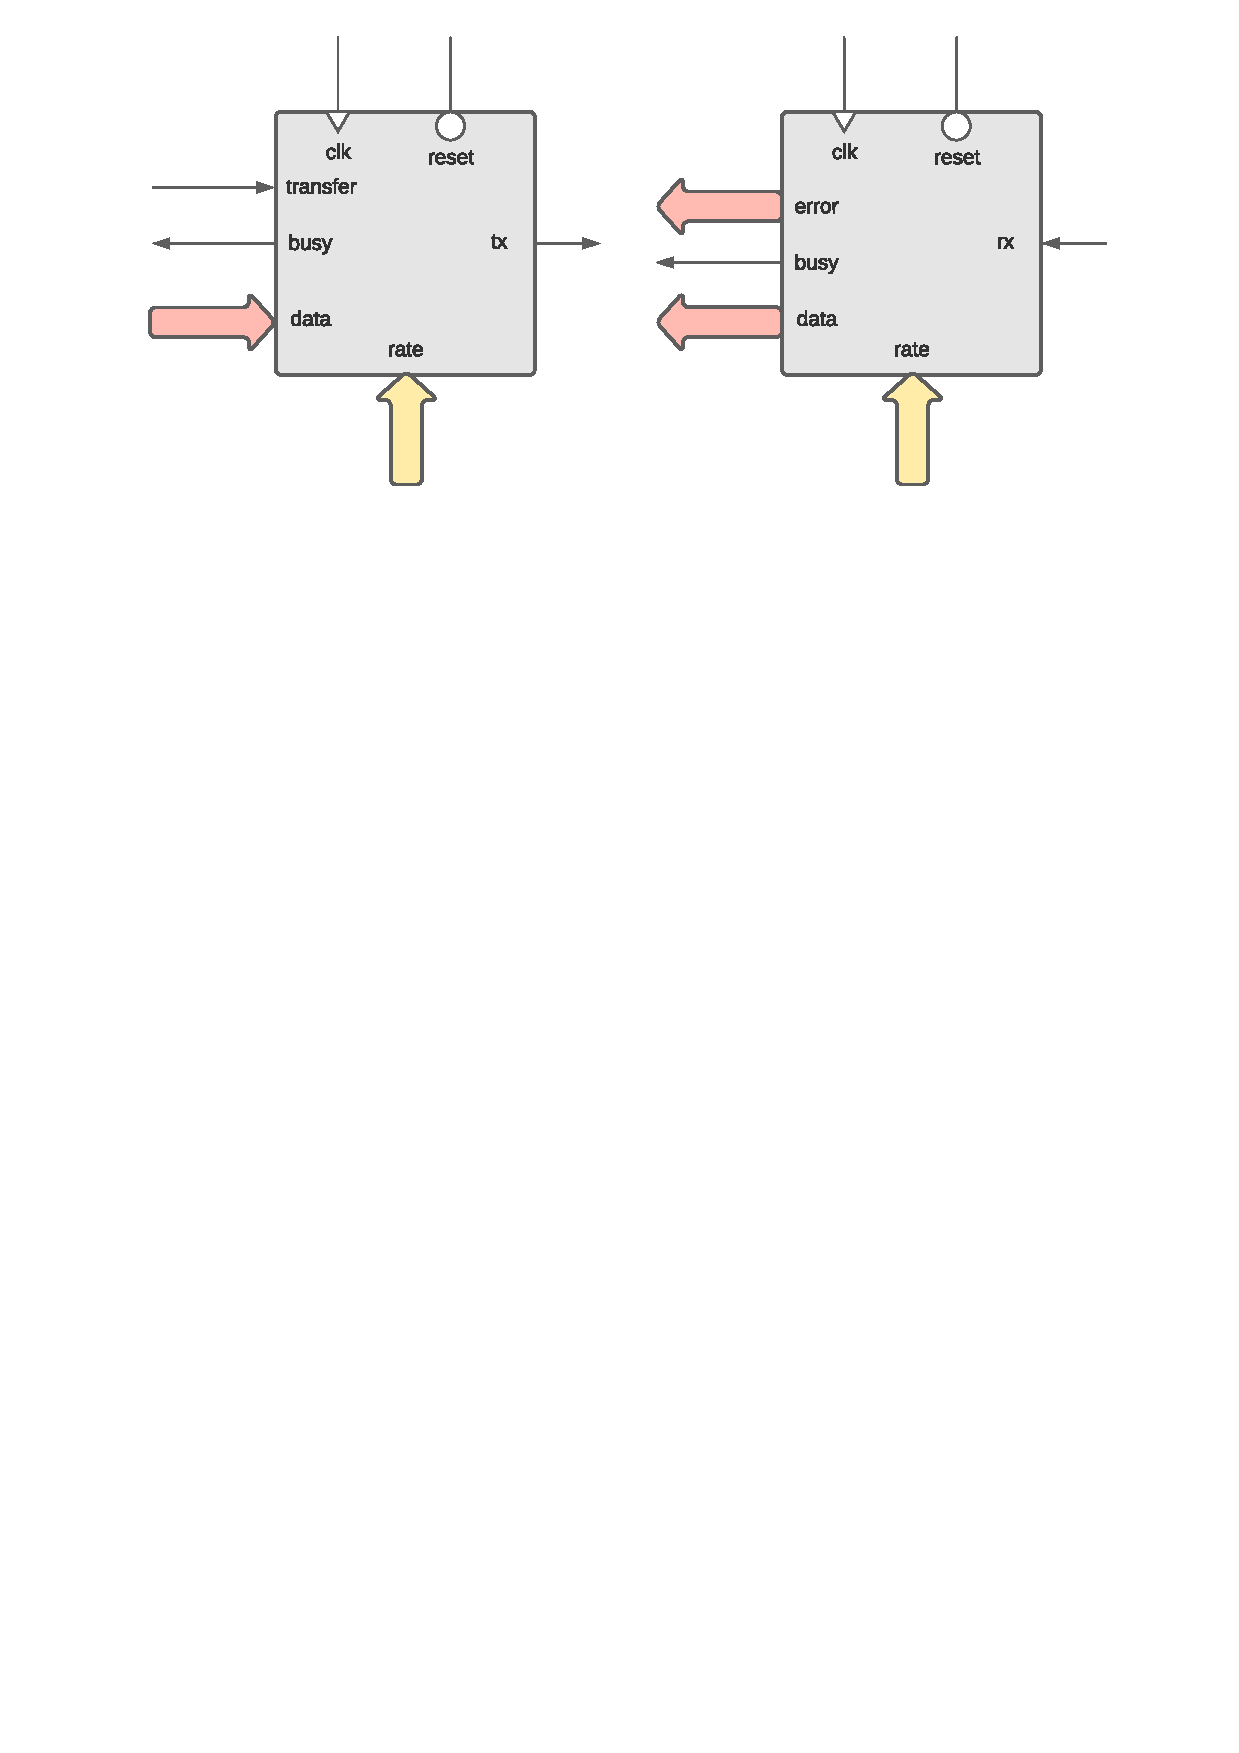
\includegraphics[scale=0.75]{img/diagrams/uart.pdf}
    \captionsetup{format=plain,justification=centering}
    \caption{Struktura wyprowadzeń modułów UART TX orax UART RX}
    \label{uart-structure}
\end{figure}
\vspace{0.5cm}

Struktury \verb|entity| reprezentujące obie podjednostki wyposarzono w~identczny zestaw parametrów (ang. \textit{generic}). Pozwalają one określić szerokość portu \verb|rate| i~format przesyłanych danych (liczbę bitów danych i~stopu oraz rodzaj parzystości). Przy ich pomocy możliwe jest też zanegowanie sygnału transmisyjnego tak, aby bezczynność linii transmisyjnej symbolizowana była stanem wysokim oraz (niezależne) zanegowanie bitów danych. W~projekcie wykorzystane zostały oba rodzaje negacji. 

Obie jednostki zostały zaimplementowane jako synchroniczne automaty skończone o~pięciu stanach. Pierwszy z~nich - \textit{idle} - przyjmowany jest w~momentach bezczynności, tj. gdy moduł oczekuje na wykrycie stanu aktywnego linii odbiorczej lub linii \verb|transfer|. W~momencie zajścia warunków startu automat przechodzi w~stan odbioru/transmisji bitu startu. Przy przejściu tym resetowany jest wewnętrzny licznik długości znaku oraz ustawiana jest linia \verb|busy|. Wartość znajdujące się na wejściu \verb|rate| zapisywana jest w~wewnętrznym buforze. W~przypadku transmisji zapisywana jest także wartość na wejściu \verb|data| a~stan linii \verb|tx| zmieniany jest na aktywny. Rzeczony licznik inkrementowany jest następnie o~jeden w~każdym następnym cyklu zegara systemowego. Moduł odbiorczy oczekuje aż jego wartość dojdzie do połowy zapisanej wartości \verb|rate| (powiększonej o~1), a~następnie próbkuje stan linii \verb|rx| w~celu zweryfikowania stanu bitu startu. Moduł nadawczy czeka natomiast czas dwukrotnie dłuższy. W~przypadku obu jednostek sytuacje te wiążą się z~przejście do kolejnego stanu - odbioru/transmisji bitów danych. Przejście do wszystkich kolejnych stanów (odbioru/nadawania bitów danych, parzystości i~stopu) wiąże się ze zresetowaniem licznika długości trwania znaku. W~przypadku odbioru bitów startu, stopu oraz parzystości odbywa się także ewentualne ustawieniem odpowiedniej flagi błędu w~wewnętrznym buforze. Przejścia do kolejnych stanów wywoływane są osiągnięciem wartości \verb|rate| przez licznik. W~następnym cyklu po odebraniu/nadaniu wszystkich bitów, stan linii \verb|busy| ustawiany jest na niski, a~dane i~flagi błędu (w~przypadku odbioru) kopiowane są z~wewnętrznych buforów na wyjście.

Dla każdego modułu stworzona została symulacja mająca na celu zweryfikowanie poprawności działania. W~jej ramach zostały stworzone procedury biblioteczne realizujące niezależnie funkcjonalność transmisji/odbioru, których kod został oparty na materiałach udostępnionych w~trakcie wykładów. Posiłkowanie się nimi miało na celu eliminację potencjalnych błędów w~procesie weryfikacji.

\vspace{0.5cm}
\begin{figure}[ht]
    \centering
    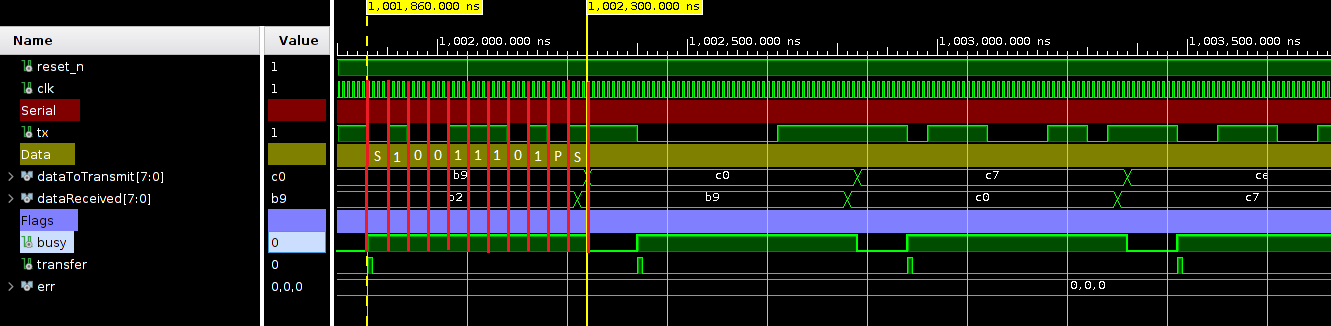
\includegraphics[scale=0.7]{img/sim/communication/uart_tx_sim.png}
    \captionsetup{format=plain,justification=centering}
    \caption{Wycinek sumylacji modułu UART TX}
    \label{sim-uart-tx}
\end{figure}
\vspace{0.5cm}

Symulacje miały charakter całościowy, tj. przetestowane zostały wszystkie kombinacje bitów transmitowanego słowa. Na Rys. \ref{sim-uart-tx} przedstawiono wycinek symulacji modułu TX. Transmitowane dane mają w~tym przypadku format 8E1. Prędkość transmisji to 25MHz natomiast prędkość zegara systemowego to 100MHz. Zastosowano tu zarówno negację sygnału jak i~danych. Pionowe linie w~kolorze czerwonym rozmieszczone zostały w~odstępach czterech cykli zegara systemowego, co odpowiada długości trwania transmitowanego bitu. Przedziadziały oznaczone literami S~odnszą się kolejno do bitu startu oraz bitu stopu. Zgodnie z~oczekiwaniami odpowiadający im stan linii \verb|tx| to odpowiednio niski i~wysoki. Bity danych to kolejno $10011101$. Po odwróceniu ich klejności (słowa transmitowane są w~kolejonści od najmniej do najbardziej znaczącego bitu) otrzymujemy $10111001$. Dane te zapisane w~formacie heksadecymalnym mają postać $0$x$B9$. Identyczna wartość ukazana jest na obrazie symulacji w~wierszu \verb|dataToTransmit|\footnote{Wysyłane słowo były wektorami losowymi z~realizacji rozkładu jednostajnego implementowanego za pomoca funkcji \textit{uniform} biblioteki \textit{math\_real}}, który obrazuje aktualnie transmitowane słowo. Oznacza to, że bity danych zostały nadane poprawnie. Bit parzystości ustawiony jest w~stanie niskim. Biorą pod uwagę nieparzystą liczbę jedynek w~przesyłanym słowie oraz negację sygnału i~danych można stwierdzić, że również ten bit został przesłany poprawnie. Sygnał \verb|dataReceived| jest ustawiany na wartość odebraną przez ww. funkcję biblioteczną. Jak widać, jego wartość zmienia się na oczekiwaną ($0$x$B9$) w~momencie połowy trwania bitu stopu. Na rysunku zaznaczone zestały także momenty ustawienia i~zresetowania stanu linii \verb|busy|. Różnica między nimi opiewa na $440$ ns. Jest to również wartość oczekiwana, ponieważ czas trwania pojedynczego bitu wynosi $40$ ns (cztery takty zegara systemowego) a~sumaryczna liczba transmitowanych bitów to $11$ ($1 + 8 + 1 + 1$). Aby ułatwić weryfikację działania modułu symulacja zostałą zaprojektowana tak, aby w~momencie niezgodności odbieranego znaku z~sygnałem \verb|dataToTransmit| stan bitów linii \verb|dataReceived| ustawiany był na $X$ reprezentowany w~symulacji kolorem czerwonym.

\vspace{0.5cm}
\begin{figure}[ht]
    \centering
    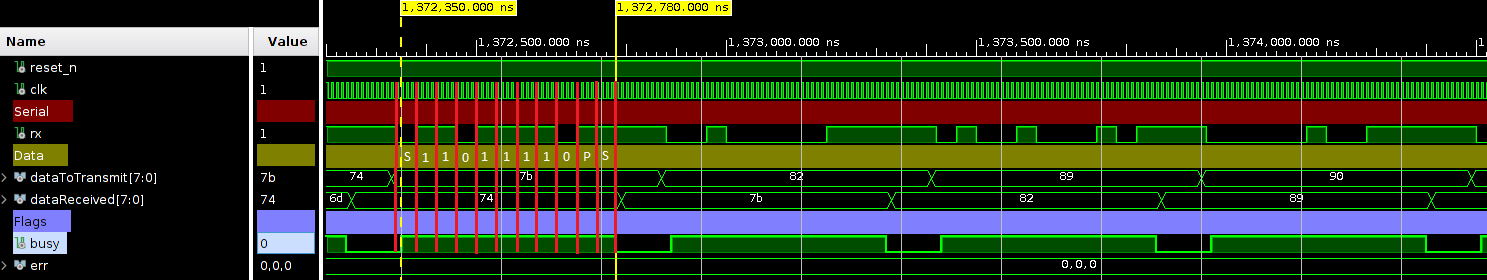
\includegraphics[width=\textwidth]{img/sim/communication/uart_rx_sim.png}
    \captionsetup{format=plain,justification=centering}
    \caption{Wycinek sumylacji modułu UART RX}
    \label{sim-uart-rx}
\end{figure}
\vspace{0.5cm}

Wycinek analogicznej symulacji dla modułu RX (przeprowadzonej przy tych samych parametrach transmisji) został zaprezentowany na Rys. \ref{sim-uart-rx}. Ponowienie analizy przeprowadzonej dla przypadku transmisji pozwala stwierdzić, że również odbiór danych odbywa się prawidłowo. Warto zauważyc, że czas wysoki na linii \verb|rx| trwa o~10 ns krócej, niż w~poprzednim przypadku. Wynika to z~faktu, że automat skończony modułu RX wychodzi ze stanu \textit{idle} dopiero w~momencie odczytania stanu aktywanego na linii odbiorczej\footnote{Po przygotowaniu grafik do sprawozdania zauważono, że moduł RX czeka o~jeden takt zegara za długo na wystawienie odberanych danych (które są gotowe już w~połowie trwania ostatniego bitu stopu). Błąd ten wynikał z~ustawienia niewłaściwego momentu próbkowania bitu startu, który przesuwał pozostałe chwile próbkowania. Został on poprawiony.}.

Przeprowadzone symulacje pozwoliły poprawić początkowe błędy implementacji a~tym samym przejść do kolejnego etapu projektowania interfejsu komunikacyjnego. Było nim stworzenie jednostek akumulujących odbierane i~transmitowane słowa do postaci N-bajto- wych próbek (określanych niżej mianem \textit{SampleTx} i~\textit{SampleRx}). Ich interfejs jest niemal identyczny jak ten przedstawiony na Rys. \ref{uart-structure}. Jedynymi różnicami są szerokość portów \verb|data| oraz brak portów wejściowych \verb|rate|. Szybkość transmisji jest w~ich przypadku ustalana poprzez parametry (\textit{generic}). Wzbogacają one interfejs UART o~dodatkowy N-bajtowy bufor wraz z~multiplexerem o~N~8-bitowych wejściach, którego wyjście połączone jest z~portem \verb|data| wewnętrznej instancji podjednostki UART TX/RX. Układy te pozwalają na odbiór/transmisję próbek w~formacie \textit{little endian} wybranym ze względu na wykorzystanie w~projekcie komputera opartego o~architekturę x86-64. Również w~ich przypadku zaprojektowane zostały symulacje mające na celu sprawdzenie poprawności dekompozycji słów na kolejno wysyłane/odbierane bajty. Filozofia ich działania jest również analogiczna do tej przedstawionej powyżej. Funkcjonalność komplementarna względem testowanego modułu jest implementowana poprzez wykonane wcześniej funkcje biblioteczne wzbogcone o~logikę pozwalającą operować na N-bajtowych słowach. Aktualnie wysyłane dane mogą być obserwowane na symulacji jako sygnał \textit{sampleToTransmit}, natomiast dane odebrane jako sygnał \textit{sampleReceived}. Jeden z~nich ustawiany jest zawsze przez moduł testowany, a~drugi przez proces wywołujący funkcję biblioteczną. Wycinek rzeczonych sumlacji dla przypadku $N=2$ został zaprezentowany na Rys. \ref{sim-sample-trensreceiver}. Niezgodność danych odbieranych z~danymi wysyłanymi lub błąd odbioru sygnalizowane są ponownie ustawieniem bitów sygnału \textit{sampleReceived} w~stan $X$.

\vspace{0.5cm}
\begin{figure}[ht]
    \centering
    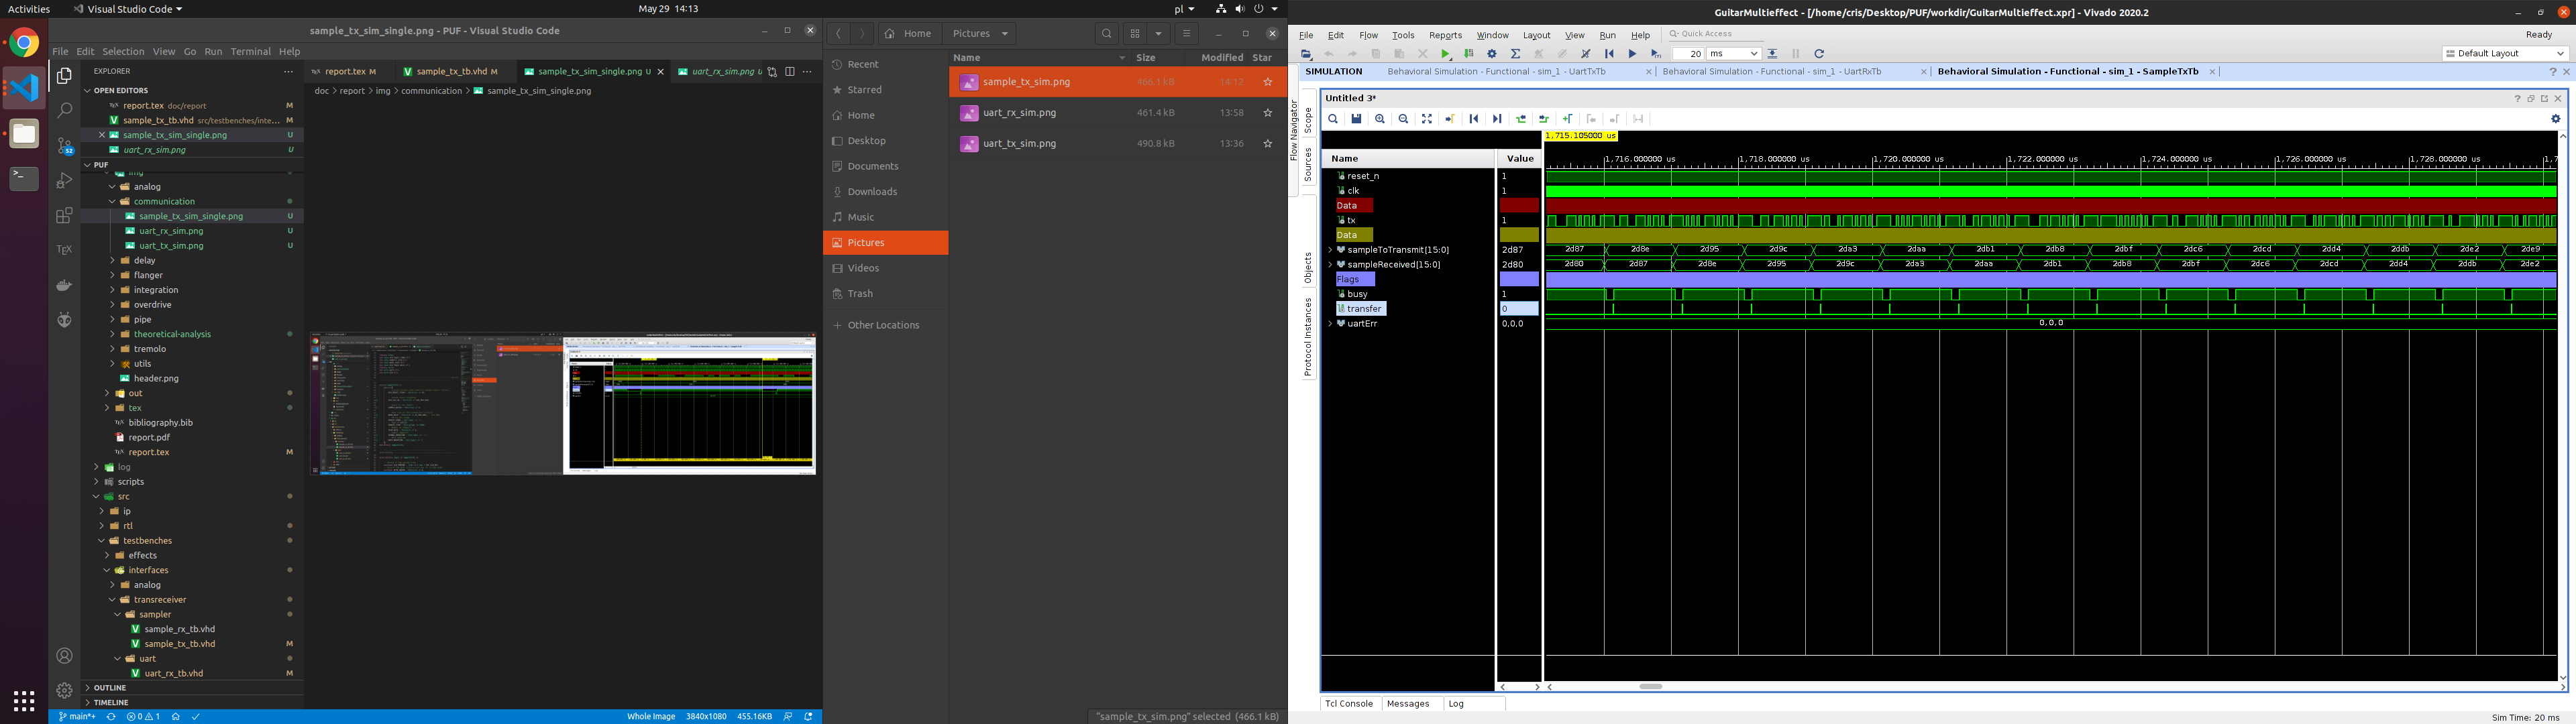
\includegraphics[width=\textwidth]{img/sim/communication/sample_tx_sim_multiple.png}
    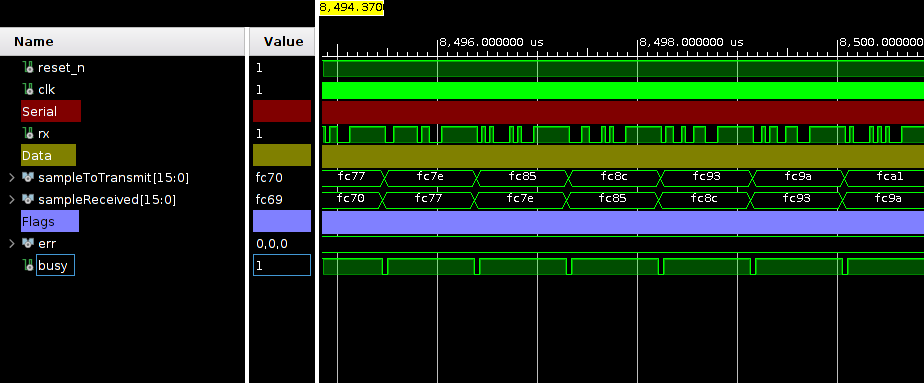
\includegraphics[width=\textwidth]{img/sim/communication/sample_rx_sim_multiple.png}
    \captionsetup{format=plain,justification=centering}
    \caption{Wycinek sumylacji modułów \textit{SampleTx} (u~góry) i~\textit{SampleRx} (u~dołu)}
    \label{sim-sample-trensreceiver}
\end{figure}
\vspace{0.5cm}

\section{Interfejs analogowy}

Drugą z~zaimplementowanych sekcji projektu był interfejs analogwy, który umożliwić miał odczyt wartości napięć na~potencjometrach z~wykorzystaniem zewnętrznego multipleksera analogowego. Zdecydowano się wykorzystać w~tym celu generator IPC (ang. \textit{Intelectual Property Core}) \textit{XADC Wizard} (wersja 3.3). Prace rozpoczęto od zapoznania się zarówno z~dokumentacją modułu ADC dostępnego w~układach FPGA serii sióddmej (\cite{xilinx_adc_series_seven}) jak i~samego generatora (\cite{xilinx_xadc_wizard}). Z~ich pomocą udało się rozszyfrować znaczenie poszczególnych parametrów rdzenia. Zdecydowano się na wykorzystanie interfejsu DRP (ang. \textit{Dynamic Reconfigurable Port}) ze względu na jego relatywną prostotę. XADC został skonfigurowany w~trybie sekwencyjnym (ang. \textit{channel sequencer}) z~manualnym wyzwalanym (ang. \textit{event mode}). Prędkość sygnału zegarowego przyjęto na poziomie 100MHz (zgodnie z~założeniami projektu) natomiast częstotliwość konwersji na poziomie 50KSPS (ang. \textit{KiloSamples Per Second}). Dodatkowo skorzystano z~udostępnianej przez XADC możliwości automatycznego wysterowania linii \textit{select} zewnętrznego multipleksera analogowego. Jako kanał roboczy wybrano \textit{vaux0}, który skonfigurowano w~trybie unipolarnym. Zrezygnowano z~uśredniania wartości próbek w~kanałach oraz dezaktywowano wszystkie alarmy. Ostatnim krokiem było ustawienie odpowiednich wartości w~sekcji \textit{Analog Sim Options} zakładki \textit{Basic}. Wpisano w~niej ścieżkę do zewnętrznęgo pliku zawierającego przebiegi symulowanych wartości analogowych. Jak się później okazało sfinalizowanie tej konfiguracji celem uzyskania możliwości uruchomienia rzeczonej symulacji, wymagało spędzenia dodatkowych kilku godzin na przeglądaniu forum \verb|forum.xilinx.com| celem odszukania informacji brakujących w~dokumentacji.

\vspace{0.5cm}
\begin{figure}[ht]
    \centering
    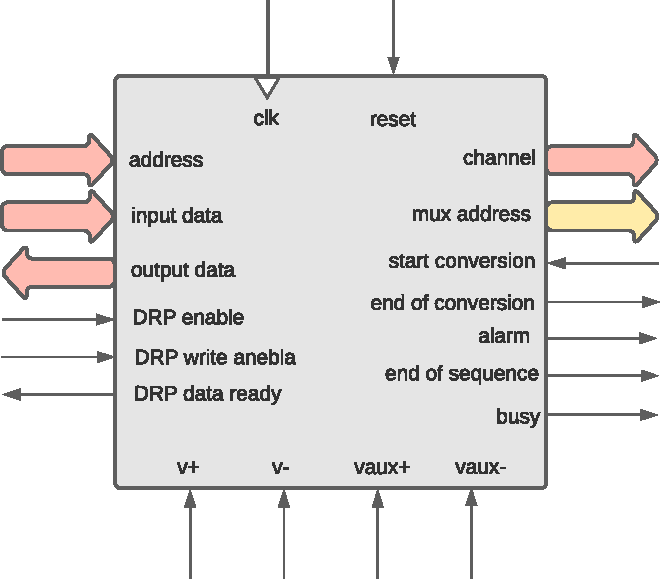
\includegraphics[scale=0.8]{img/diagrams/xadc.pdf}
    \captionsetup{format=plain,justification=centering}
    \caption{Struktura portów wygenerowanego modułu XADC}
    \label{xadc-structure}
\end{figure}
\vspace{0.5cm}

Strukturę wyprowadzeń wygenerowanego bloku funkcjonalnego przedstawiono na Rys. \ref{xadc-structure}. Po lewej stronie przedstawiono sygnały związane z~odczytem i~zapisem wewnętrznych rejestrów modułu. Na dolnej krawędzi znalazły się bipolarne wejścia analogowe. Znaczenie sygnałów zaprezentowanych naprawej krawędzi są następujące:

\begin{itemize}
    \item \textit{channel} - port wyjściowy reprezentujący adres rejestru zawierającego dane z~ostatniego kanału spróbkowanego przez XADC; ustawiany jest na końcu konwersji (niewykorzystany w~projekcie)
    \item \textit{mux address} - linie wysterowujące wejścia \textit{select} zewnętrznego multipleksera analogowego
    \item \textit{start conversion} - linia aktywujące nową konwersję
    \item \textit{end of conversion} - linia ustawiana w~stan wysoki na jeden takt zegara po zakończeniu konwersji
    \item \textit{alarm} i~\textit{end of sequence} - linie alaramu oraz sygnalizacji końca sekwencji aktywne w~stanie wysokim (nieużywane w~projekcie)
    \item \textit{busy} - linia ustawiana w~stan wysoki na czas trwania konwersji
\end{itemize}

Wokół tak przedstawiającej się struktury stworzony został prosty moduł interfejsujący, który automatyzuje cykliczne wyzwalania konwersji oraz odczyt danych z~wewnętrznych rejestrów XADC. Jego struktura została przedstawiona na Rys. \ref{analog-scanner-structure}. Port \verb|data| reprezentowany jest przez tablicę N~wektorów 12-bitowych ($N <= 16$) odzwierciedlających wartości napięcia na kolejnych kanałach multipleksera. W~projekcie wykorzystano dziewięć kanałów (dziewięć potencjometrów), których znaczenie przedstawiono w~dalszej części dokumentu. Na zewnątrz modułu wystawione zostały poza tym wejścia analogowe kanału \textit{vaux0} (oznaczone omyłkowo jako wyjścia) oraz linie \textit{select} dla zewnętrznego multipleksera. Dedykowane wejścia analogowe (\textit{vp/vn}) zostały podłączone na stałe do masy. Parametry (ang.\textit{generic}) modułu pozwalają skonfigurować ilość wykorzystywanych kanałów\footnote{Musi być zgodna z~konfiguracją podaną na etapie generowania XADC} oraz częstotliwość ich próbkowania.
 
\vspace{0.5cm}
\begin{figure}[ht]
    \centering
    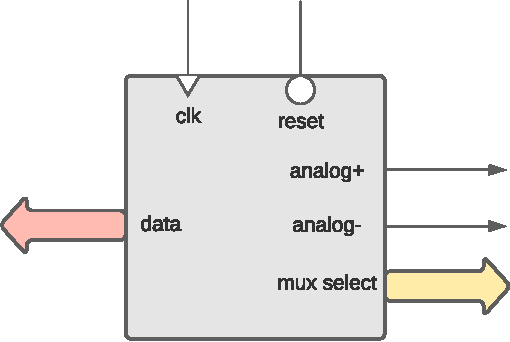
\includegraphics[scale=1.0]{img/diagrams/analog_scanner.pdf}
    \captionsetup{format=plain,justification=centering}
    \caption{Struktura portów bloku skanera kanałów analogowych}
    \label{analog-scanner-structure}
\end{figure}
\vspace{0.5cm}

Zasada działania modułu zasadza się na dwóch synchronicznych procesach. Pierwszy z~nich wyposażony jest w~wewnętrzny licznik, który odmierza takty zegara systemowego między kolejnymi konwersjami. Gdy jego wartość spadnie do zera linia \verb|start conversion| bloku XADC zostaje ustawiona w~stan wysoki na jeden cykl zegara. Równolegle wartość wyjścia \verb|mux address| - powiększona o~wartość $0$x$10$ (adres danych pierwszego kanału pomocniczego \textit{vaux0}) - zostaje przepisana na wejście adresowe interfejsu DRP. Drugi proces implementuje dwustanowy automat skończony. W~pierwszym ze stanów proces oczekuje na pojawienie się logicznej jedynki na linii \verb|end of conversion|. Gdy sytuacja ta zajdzie, linia \verb|DRP enable| również ustawiana jest w~stan wysoki, co rozpoczyna odczyt danych spod adresu znajdującego się na liniach adresowych (ustawianych przez pierwszy proces). Akcja finalizowana jest przejściem do drugiego stanu, w~którym proces pozostaje do wystawienia przez XADC logicznej jedynki na linii \verb|DRP ready| oznaczającej pojawienie się odczytanych danych na procie \verb|output data|. Dane te kopowiane są do odpowiedniego wektora w~tablicy \verb|data| i~proces przechodzi ponownie do stanu pierwszego.

W~celu weryfikacji zaimplementowanego rozwiązania ponownie przygotowano stosowną symulację. Tym razem weryfikacja nie miała charakteru formalnego, tzn. efekty działania testowanego modułu nie były programowo porównywane z~wartościami oczekiwanymi. Ze względu na złożoność implementacji takiego rozwiązania ograniczono się jedynie do weryfikacji jakościowej poprzez manualną analizę zasymulowanych przebiegów. Aby jednak symulacja była możliwa należało najpierw stworzyć odpowiedni plik zawierający przebiegi wartości napięcia na kolejnych kanałach ADC. Generację takowego pliku zautomatyzowano za pomocą prostego skryptu języka Python, który pozwala zdefiniować długość trwania generowanych sygnałów, ich przebieg oraz częstotliwość ``próbkowania''. Z~jego pomocą wygenerowano sinusoidalny przebieg napięcia na kanale \textit{vauxp0} ustawiając jednocześnie pozostałe kanały na wartość~$0$. Fragment symulacji obrazuje Rys. \ref{sim-analog-scanner}. Przyjęto w~niej częstotliwość konwersji na maksymalnym poziomie 50KSPS. Jak widać wektory tabeli \textit{channels\_out} (podłączej do portu wyjściowego \verb|data| skanera) są aktualizowane w~zakładany sposób. Dla lepszego zobrazowania sposobu działania układu rysunek ukazuje także bezpośrednie przebiegi niektórych portów modułu XADC. 

\vspace{0.5cm}
\begin{figure}[ht]
    \centering
    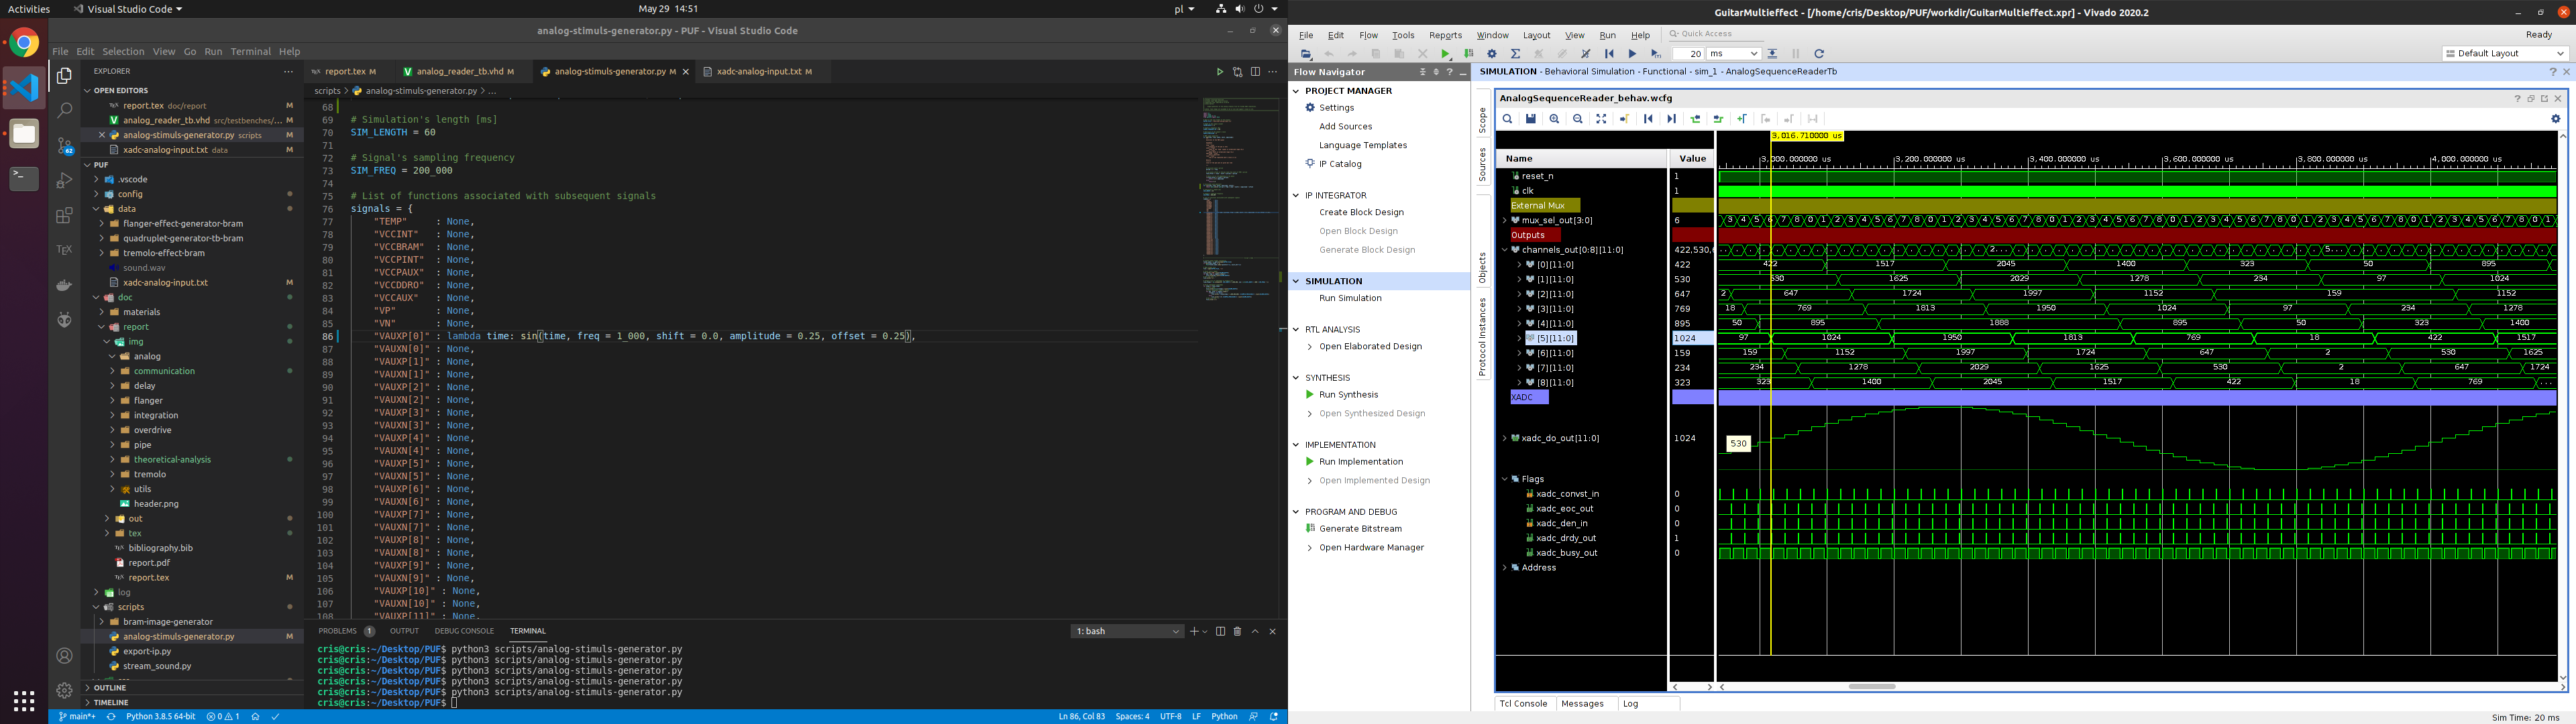
\includegraphics[width=\textwidth]{img/sim/analog_scanner_sim.png}
    \captionsetup{format=plain,justification=centering}
    \caption{Fragment symulacji bloku skanera analogowego}
    \label{sim-analog-scanner}
\end{figure}
\vspace{0.5cm}


% Bibliography
\clearpage
\printbibliography

\end{document}


